\chapter{Methods}\label{chap:methods}

The primary methodology employed in this thesis to assess the quality of metrics
used to evaluate generative protein models is heavily inspired by
\cite{obray2022evaluation}, and consists in evaluating how well a particular
combination of representation, optional descriptor function, kernel and
parameters applied to all three aforementioned elements\footnote{We also
subsequently refer to the parametrization and choice of all these options as an
\acrshort{mmd} \emph{configuration}.} correlates with the amount of
perturbation % TODO: check with Tim to see if use of term configuration is OK.
applied to one set of proteins. This can be broken down in the following steps:

\begin{enumerate}
\item Take two i.i.d. samples from a database of proteins.
\item Progressively perturb to one of the samples.
\item Measure the \acrshort{mmd} between the unperturbed and perturbed sample.
\item Once the varying degrees of perturbations have been applied and
accompanying \acrshort{mmd}s catalogued, compute the correlation coefficient
between the \acrshort{mmd} and the amount of perturbation.
\end{enumerate}

A particular MMD configuration is considered superior to another if the
resulting correlation coefficients of the former are higher than that of the latter.

In this chapter, we start by motivating the datasets that will be used to simulate a generative
protein model. We then describe and motivate the experimental setups -- i.e.
perturbations -- that we will employ to test the various configurations of \acrshort{mmd}.
Finally, we enumerate and justify which configurations of \acrshort{mmd} are tested,
including all the combinations of protein representations, descriptor functions,
and kernels. Finally, we describe and motivate the experimental setups -- i.e.
perturbations -- that we will employ to test the various metric configurations.

\section{Datasets}

In this thesis, except otherwise stated, all results will be derived from 10
random samples from the \textit{homo sapiens} monomeric proteome downloaded from
the EBI AlphaFold2 database
\citep{varadi2022alphafold,tunyasuvunakool2021highly}, a repository comprising
predicted 3D structures of protein sequences obtained from AlphaFold2, the
current state-of-the-art method to predict protein structure from sequences
\citep{jumper2021highly}. Multiple reasons justify this choice. First, despite
being a proxy for experimentally validated proteins, AlphaFold2 is known to
provide predicted 3D structures for naturally occurring proteins with the same
accuracy as experimentally acquired 3D structures \citep{jumper2021highly},
ensuring that the conclusions we reach in this thesis will be broadly applicable
to experimentally acquired protein structures. Second, this allows us to
establish the ground truth of a range of \acrshort{mmd} configurations, hence
also enabling the gauging the quality of Third, there are practical advantages
related to this database because it contains consistently formatted \texttt{pdb}
files exclusively cataloguing heavy atoms directly contributing to the 3D
structure of a single monomer, which simplifies downstream processing.
% TODO: not sure what was meant in the reasonable generated samples (2nd
% reason).

\section{Perturbations}

While \cite{obray2022evaluation} focused on \emph{graph perturbations} specifically,
we wanted to augment and refine the set of perturbations applied to the perturbed
sample of proteins to be more pertinent to proteins. Three
categories of perturbations can be distinguished:

\paragraph{Graph Perturbations} These perturbations mostly overlap with those
defined by \cite{obray2022evaluation}, as they include (i) adding edges to a graph
(ii) removing edges from a graph, and (iii) rewiring, i.e. swapping, edges within a
graph.
\paragraph{Point Cloud Perturbations} These perturbations aim to add changes
to the underlying coordinates of each atom in the protein. Such
perturbations include injecting Gaussian noise (Equation
\ref{eq:gaussian_noise}), (ii) twisting, (iii) shearing, and
(iv) tapering. Importantly, where appropriate, we extract the graphs \emph{after} applying the
point cloud perturbation, to ensure the changes in the point cloud can be
reflected in the graph structure. We proceed to detail each of the equations governing the
perturbations below. An illustration of each of those perturbations can be found
in Figure \ref{fig:perturbation_illustration}

In the notation that follows, $x$, $y$ $z$ represent the unperturbed coordinates, and
$x'$, $y'$, and $z'$ represent the perturbed coordinates. The \emph{Gaussian noise} added to a coordinate system is given by:
\begin{equation}
  \label{eq:gaussian_noise}
  \begin{bmatrix}
    x' \\
    y' \\
    z'
  \end{bmatrix} =
  \begin{bmatrix}
    x+ \text{Noise} \\
    y+ \text{Noise} \\
    z+ \text{Noise}
  \end{bmatrix}
\end{equation}
where $\text{Noise}\sim\caln(0,\sigma)$ and $\sigma$ is set by the user.
\emph{Twisting} is achieved by adding the following transformation to the coordinate
system:

\begin{equation}
  \label{eq:twisting}
  \begin{bmatrix}
    x' \\
    y' \\
    z'
  \end{bmatrix} =
  \begin{bmatrix}
    x\cdot\cos(\alpha\cdot z) - y\cdot\sin(\alpha\cdot z) \\
    x\cdot\sin(\alpha\cdot z) + y\cdot\sin(\alpha\cdot z) \\
    z
  \end{bmatrix}
\end{equation}

where $\alpha\in\R$ is in $\rad\cdot\si{
\angstrom}^{-1}$ is set by the user. \emph{Shearing} the coordinate system is achieved
by applying

\begin{equation}
  \label{eq:shearing}
  \begin{bmatrix}
    x' \\
    y' \\
    z'
  \end{bmatrix} =
  \begin{bmatrix}
    a \cdot z + x\\
    b \cdot z + y\\
    z
  \end{bmatrix}
\end{equation}

to the coordinate system, where $a, b\in\R$ are in \si{\angstrom} and set by the user. In this thesis, we set $a=b$. Similarly,
\emph{tapering} is achieved by applying


\begin{equation}
  \label{eq:tapering}
  \begin{bmatrix}
    x' \\
    y' \\
    z'
  \end{bmatrix} =
  \begin{bmatrix}
    (0.5\cdot a^2\cdot z + b\cdot z + 1) \cdot x\\
    (0.5\cdot a^2\cdot z + b\cdot z + 1) \cdot y\\
    z
  \end{bmatrix}
\end{equation}

where $a, b\in\R$ are in \si{\angstrom} and set by the user. Similarly to
Equation \ref{eq:shearing}, we set $a=b$ in this thesis.

\begin{figure}
  \centering
  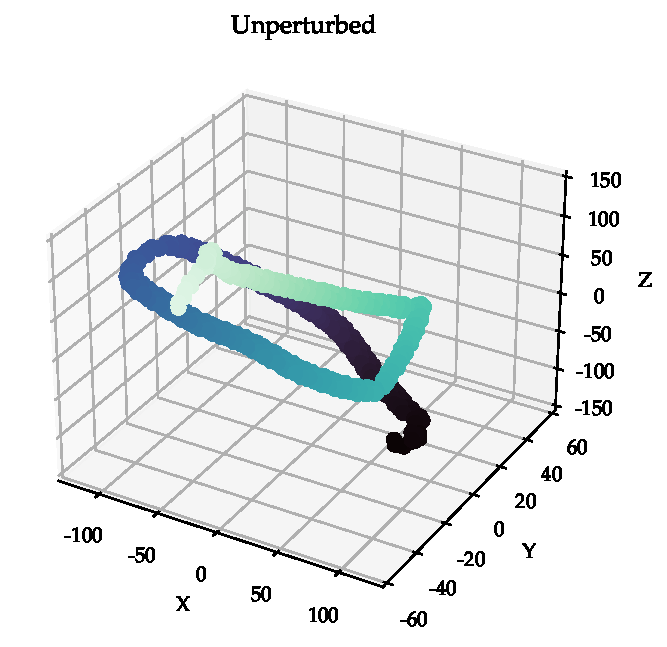
\includegraphics[width=0.5\textwidth]{./figures/protein_unperturbed.pdf}
  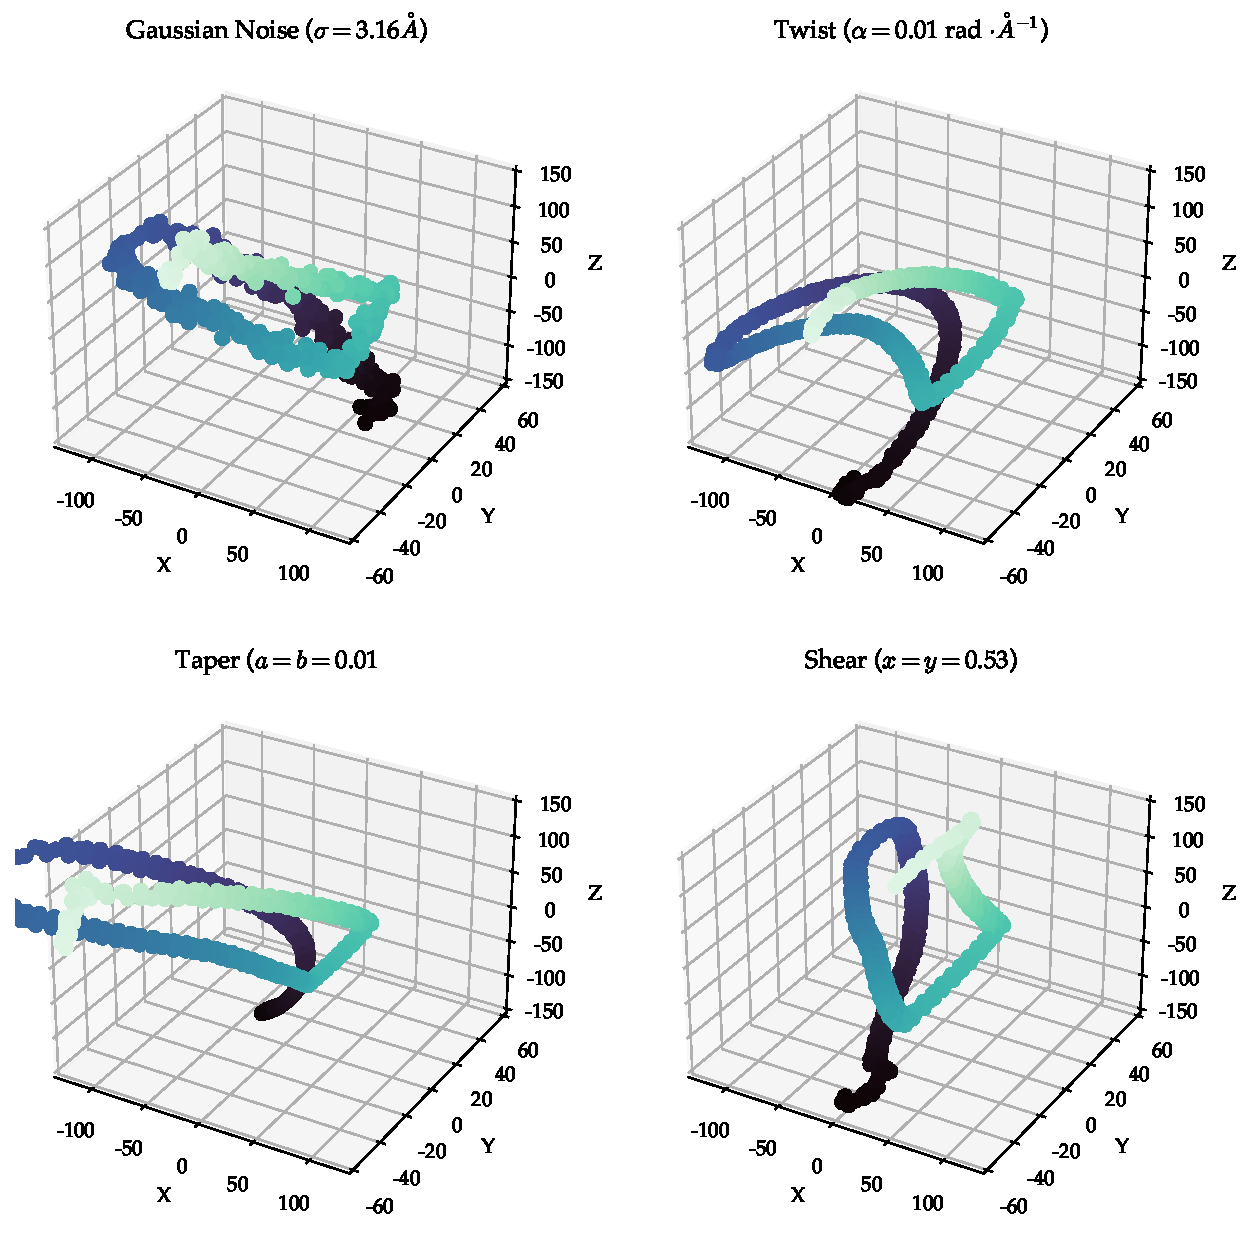
\includegraphics[width=\textwidth]{./figures/protein_perturbed.pdf}
  \caption[Illustration of all point cloud perturbations applied to a
protein.]{Illustration of all point cloud perturbations applied to a protein.
The amount of each perturbation shown here corresponds to 10\% of the maximum
value of the maximum value of each perturbation as shown in Table
\ref{tab:perturbation_ranges}. The protein displayed here is the cilia- and
flagella-associated protein 53 (UniProt code Q96M91). Each $\alpha$ carbon is
colored according to its position on the chain. On the unperturbed protein, the
lighter colors are located closer to the viewer.}
  \label{fig:perturbation_illustration}
\end{figure}

\paragraph{Mutation} These simply consist in (i) selecting the positions that
will be mutated by sampling from a Bernoulli distribution with parameter $p$ and
(ii) for selected positions, swap the amino acid by any of the 20 possible
naturally-occurring amino acids. While graph perturbation probabilities (e.g. of
adding an edge) range from 0 to 1, here we mostly concentrate on lower regimes
of mutation, i.e. between 0 and 0.1, so see how sensitive various \acrshort{mmd}
configurations are to a few point mutations, which covers most of the
real-world % TODO: some -> most OK?
protein engineering use cases \citep{poluri2017protein}.

For each perturbation, a range of degrees of perturbation is defined and 20
different evenly-spaced degrees of perturbation are examined and repeated 10
times with 10 pairs of i.i.d. proteins to estimate the sensitivity of the
particular \acrshort{mmd} configuration to the perturbation. The ranges used for each
parameter used in this thesis are shown in Table \ref{tab:perturbation_ranges}


\begin{table}
  \centering
  \begin{tabular}{>{\raggedright\arraybackslash}p{4.8cm}l}
    \toprule
    \textbf{Perturbation} & \textbf{Range} \\
    \midrule
    Twist & [0, 0.1] (rad/\si{\angstrom})\\
    Shear & [0, 5] (\si{\angstrom}) \\
    Taper & [0, 0.1] (\si{\angstrom}, \si{\angstrom}) \\
    Gaussian Noise & [0, 30] (\si{\angstrom}) \\
    Mutation & [0, 0.1]\\
    Graph Perturbations (remove, add, rewire edges) & [0, 1]\\
    \bottomrule
  \end{tabular}
  \caption[Perturbation ranges used in this thesis.]{Perturbation ranges used in this thesis. Each interval was split into
    20 evenly-spaced degrees of perturbation.}
  \label{tab:perturbation_ranges}
\end{table}

\section{MMD Configurations}

We introduced \acrshort{mmd} in Section \ref{sec:mmd} (Equation \ref{eq:mmd} and
\ref{eq:mmd_unbiased}), and noted that an important aspect of using
\acrshort{mmd} in practice consists in choosing the right descriptor function
and kernel, because it heavily impacts which aspects of the data are distilled
for analysis in MMD and also heavily impacts how the data is processed by the
kernel functions inside of MMD. Here, we list and motivate all graph extraction
techniques, descriptor functions employed, and kernels adopted in this
experiment.

First, throughout our experiments, we will use the unbiased squared
\acrshort{mmd} estimate, which removes self-comparison terms in the kernel
matrices (\cite{gretton2012kernel}, Lemma 6), which can result in negative
values. We will normalize the resulting \acrshort{mmd} over the whole range of
perturbation for each curve as well to compare behaviors of different
\acrshort{mmd} configurations not operating on the same scale. As highlighted in
Section \ref{sec:mmd}, \acrshort{mmd} does not have an inherent sense of scale
anyway, so this normalization step does not impact our analysis negatively.
% TODO: check syntax

\begin{equation}
  \label{eq:normalization}
  \MMD_{\textnormal{Normalized}} = {\MMD - \min(\MMD_{\textnormal{Experiment}}) \over \max(\MMD_{\textnormal{Experiment}}) - \min(\MMD_{\textnormal{Experiment}})}
\end{equation}

Where $\MMD_{\textnormal{Experiment}}$ is the collection of \acrshort{mmd} values for a particular
experiment, i.e. a particular \acrshort{mmd} configuration tracked through the whole range
of a particular perturbation.

\subsection{Representations}
We will use several different representations of proteins in this thesis, which can be
grouped into three categories. The first is \emph{coordinates}. These are parsed
from each \texttt{.pdb} file. The second is \emph{graphs}. They include $k$-NN
and $\varepsilon$-graphs, introduced in Section \ref{sec:graphs}. A summary
table of the different types of graphs extracted from proteins in this thesis
can be found in Table \ref{tab:graph_extraction}. The third is the simple
protein \emph{sequence}. Each protein's sequence parsed from each \texttt{.pdb}
file as is. Since we are only dealing with monomers, no additional processing is
required.

\begin{table}
  \centering
  \begin{tabular}{ll}
    \toprule
    \textbf{Graph type} & \textbf{Values} \\
    \midrule
    $k$-NN graphs & $k\in \{2, 6, 8\}$ \\
    $\varepsilon$-graphs & $\varepsilon\in\{8, 16, 32\}$ \\
    \bottomrule
  \end{tabular}
  \caption{Ranges of parameters used to extract graphs from point clouds in this thesis.}
  \label{tab:graph_extraction}
\end{table}


\subsection{Descriptor Functions}\label{sec:descriptors}

As discussed in Section \ref{sec:mmd}, some kernels require some alternative vectorized
representation to work. We will use the following protein descriptor functions
here.


\paragraph{Graph descriptors} They are defined in Section \ref{sec:mmd} and include
  the degree distribution histogram, the clustering coefficient histogram and
  the Laplacian spectrum histogram. These are all fixed-length vectors. The
  maximum value of the degree histogram was determined based on the longest
  sequence length of the proteins in the dataset (2699), because the node degree
  of any given graph will be at most equal to the size of the largest graph in
  the dataset. This aspect is particularly relevant when considering the
  perturbation adding edges to a protein graph.

\paragraph{Coordinates descriptors} In order to capture the information of the
3D structure of the protein beyond local neighborhood information, a topological
descriptor of each protein in the form of a persistence diagram is extracted
using a Vietoris-Rips filtration introduced in detail in Section \ref{sec:tda}.
To speed up computation (and since we do not take amino acid type into account
for this analysis), we sampled every other point to dramatically reduce the
running time and memory footprint without significantly affecting the shape of
the protein. % TODO: build validation script. Ideas:% compute persistence diagrams and show similarity.

\paragraph{Protein-specific descriptors} In this thesis we introduce two novel
protein-specific descriptor functions resulting in fixed-length vector
representations for subsequent use in kernels accepting inputs in $\R^d$. The
first consists of a histogram of the pairwise distance of each
\textalpha{}-carbon\footnote{In principle, an all-atom histogram could also be
computed; we just anticipate that the added value of such an all-atom histogram
would be minimal in comparison to the significantly increase computation cost
and memory footprint of the resulting histogram.}; the second consists in
concatenating the two histograms of the two dihedral angles $\phi$ and $\psi$
formed by each amino acid discussed in Section \ref{sec:proteins}. The
inspiration behind those two descriptors comes from elements of the validation
pipeline of novel Protein Data Bank structures \citep{read2011new,
gore2012implementing, gore2017validation}, where atoms too close together are
flagged and unusual dihedral angles are reported to penalize the overall
validity of the protein 3D model to be validated. Those unusual dihedral angles
are also called ``Ramachandran outliers'', after the scientist who discovered a
way to display the $\phi$ and $\psi$ in a 2-D histogram, and recovered features
in this histogram related to the secondary structure of the protein from such
plots. \citep{ramachandran1063Stereochemistry}. Overall, both the biological
relevance and the established scientific success of distance histograms and
dihedral angles histogram in both the validation and analysis of proteins lend
credence to those newly established descriptors.

% TODO: flattened distogram?

\paragraph{Sequence descriptors} In Section \ref{sec:mmd}, we discussed the
Evolutionary Scale Modelling family to construct descriptors of a fixed length
using a learned embedding. We use the 6-layer variant trained on
the UniRef50 snapshot from March 2018 which contains approximately 43 million
parameters, because it is able to process the full range of sequence lengths
that we have in our dataset (the longest sequence fragment is 2699 amino acids long).

Table \ref{tab:descriptor_function_setup} summarizes the parameters used to set
up the descriptor functions in this thesis.

\begin{table}
  \centering
  \begin{tabular}{lll}
    \toprule
    \textbf{Descriptor Name} & \textbf{Number of Bins} & \textbf{Range of Bins} \\
    \midrule
    Degree Histogram & 2699 & [0, 2699] \\
    Laplacian Spectrum Histogram & 100 & [0, 2] \\
    Distance Histogram & 1000 & [0, 1000] (\si{\angstrom}) \\
    Dihedral Angles Histogram & 100 & [$-\pi$, $+\pi$] (rad) \\
    \bottomrule
  \end{tabular}
  \caption[Descriptor function bin numbers and ranges of descriptor functions
  used in this thesis.]{Descriptor function bin numbers and ranges of descriptor functions
    used in this thesis. The ranges are given by
    [minimum value, maximum value] and (unit) when applicable.}
  \label{tab:descriptor_function_setup}
\end{table}

% TODO: add pgfplots figure of this workflow.

\subsection{Kernels}\label{sec:methods_kernels}
Once a suitable representation and descriptor function is selected, one requires
a kernel to evaluate the \acrshort{mmd} in the corresponding \acrshort{rkhs}. We
detail which kernels we are going to evaluate and why in this section. Kernels
used in this thesis can be grouped into three separate categories.

The first category has been discussed in the literature extensively since it was
used to evaluate generative graph neural network models, i.e. the
\emph{fixed-length vector kernels} like the Gaussian (RBF) kernel and the linear
kernel, both of which are defined in Section \ref{sec:kernels}\footnote{We will
  follow the speed-up trick outlined in Appendix A.5 by \cite{obray2022evaluation}
  to reduce the computation time of each different bandwidth parameter.}. Since the only
condition for each vector to be valid inputs for those kernels is that they are
in $\R^d$, the protein-specific vector representations outlined in Section
\ref{sec:descriptors} are valid inputs.
% Special implementation of wl-k

As alluded to in Section \ref{sec:kernels}, we introduce two new classes of
kernels for use in \acrshort{mmd} which so far have not been used to evaluate generative
models due to the unique aspects of proteins that need to be captured. This
brings us to the second category of kernels used in this thesis: \emph{graph kernels}.
Specifically, we are going to use the Weisfeiler-Lehman kernel discussed in
Section \ref{sec:kernels} because it captures \emph{local} patterns in the
neighbourhood of each node. In Appendix \ref{sec:sparse_wl}, we detail how we
achieved an 80\% improvement in the runtime of the Weisfeiler-Lehman kernel by
leveraging the sparsity of the graphs used in this thesis.

To estimate \emph{global} changes in the shape of the protein, we will also use
kernels accepting persistence diagrams as input, specifically, we will adopt the
Persistence Fisher kernel \citep{le2018persistence} and the multi-scale kernel
\citep{reininghaus2015stable} defined in Section \ref{sec:kernels}.


\section{Experimental Setup}

\subsection{Measuring the Quality of \acrshort{mmd} Configurations}

To objectively evaluate the various representation, descriptor, and kernel
combinations used in \acrshort{mmd}, we will use two correlation coefficients, namely the
Spearman's correlation coefficient and Pearson's correlation coefficient, each
given by:
\begin{equation}
  \label{eq:spearman} \rho_s(X,Y) = {\cov(\rank(X), \rank(Y)) \over
\sigma_{\rank(X)}\sigma_{\rank(Y)}},
\end{equation} and
\begin{equation}
  \label{eq:pearson} \rho_p(X,Y) = {\cov(X, Y)\over \sigma_X\sigma_Y},
\end{equation}
respectively. Here, $X$ is the vector containing the set of values used to
perturb one of the protein sets and $Y$ the vector of \acrshort{mmd} values
between the unperturbed and perturbed set for each perturbation level. In this
setting, a high Spearman correlation coefficient (Equation \ref{eq:spearman}) is
crucial to satisfy the first criterium of a performance metric: expressivity
(see Section \ref{sec:evalproblem}). This will guarantee that the metric
increases monotonically with the amount of perturbation. As
\cite{obray2022evaluation} have shown, some configurations of \acrshort{mmd} on
synthetic datasets revealed that an increasing \acrshort{mmd} value with
increasing perturbation is not guaranteed. While \cite{thompson2022evaluation}
highlighted that linearity is not a requirement, the Pearson correlation
coefficient (Equation \ref{eq:pearson}) will allow us to further refine the
selection of the metrics behaving most predictably, and distill the most
relevant configurations for a given perturbation range.

Another important metric we can employ to quantify the quality of a particular
\acrshort{mmd} configuration is the standard deviation of the various
\acrshort{mmd} values across runs over the whole range of pertubations. As
indicated in Section \ref{sec:evalproblem}, one of the desiderata for a
generative model metric is robustness. Since all experiments have been run with
the same number of i.i.d. samples every time, using the standard deviation
allows us to estimate how much a particular \acrshort{mmd} configuration is sensitive
to the underlying data used. An \acrshort{mmd} configuration with a high standard
deviation under a particular perturbation regime would be indicative of low
robustness, and would therefore be a less reliable estimate of the quality of
the samples compared to an \acrshort{mmd} configuration with a high standard
deviation. We abbreviate this standard deviation measure as $\sigma_\MMD$ to
avoid confusion with the $\sigma$ parameter of the RBF kernel presented in
Section \ref{sec:methods_kernels}. In Chapter \ref{chap:results}, wherever we
conduct statistical tests, our highest significance threshold is $5\cdot 10^{-2}$.
significance threshold is


\subsection{Software Library Design}


Due to the complexity and modularity of the methodology explored above, it is
required to have a scalable library to execute all the evaluation experiments at
scale and efficiently. To accomplish this task, we developed a custom Python
library leveraging parallel processing of data to the greatest extent possible.
We were inspired by the standards of \texttt{scikit-learn} and implemented
multiple modules following the same design patterns to ensure that we could
build \texttt{Pipeline} objects with the necessary steps required to compute an
\acrshort{mmd}. All the code used for this thesis can be found here:
\url{https://github.com/pjhartout/msc_thesis}

% TODO: Plot of the library structure.

\section{Summary}

In this chapter, we detailed the methodological setup employed in this thesis.
We first described the datasets we used, as well as the type of perturbations
applied to them. We then discussed the representations of the proteins used in
this study, as well as described the descriptor functions used for those
representations. Crucially, we motivated our choice for the collection of
kernels used for estimating the \acrshort{mmd}. Finally, we outlined the
methodology leveraged to rank the quality of various \acrshort{mmd}
configurations objectively.
